\section{Machine Learning - SVM}



%\includegraphics[scale = 0.2]{scikitlearn}
\emph{Support Vector Machine} (SVM) is a tool used in machine learning for classifying data points.   For instance, if there are red and black data points, how can we find a good line that separates them?  The input data that you are given is as follows:

\paragraph{Input:}
\begin{itemize}
\item $d$-dimensional data points $x^1, \dots, x^N$ 
\item $1$-dimensional labels $z^1, \dots, z^N$  (typically we will use $z_i$ is either $1$  or $-1$)
\end{itemize}

The output to the problem should he a hyperplane $w^\top x + b = 0$ that separates the two data types (either exact separation or approximate separation).

\paragraph{Output:}
\begin{itemize}
\item A $d$-dimensional vector $w$
\item A $1$-dimensional value $b$
\end{itemize}

Given this output, we can construct a classification function $f(x)$ as 

\begin{equation}
f(x) = \begin{cases}
1 & \text{ if } w^\top x + b \geq 0,\\
-1 & \text{ if } w^\top x + b < 0.
\end{cases}
\end{equation}


\begin{general}{Support Vector Machine - Exact Classification}{}
Given labeled data $(\mathbf{x}^i, y_i)$ for $i=1, \dots, N$, where $\mathbf{x}^i \in \R^d$ and $y^i \in \{-1,1\}$, find a vector $\mathbf{w} \in \R^d$ and a number $b \in \R$ such that 
\begin{align}
\mathbf{x}^i \cdot \mathbf{w} + b & > 0  & \text{ if } y^i = 1\\
\mathbf{x}^i \cdot \mathbf{w} + b & < 0  & \text{ if } y^i = -1
\end{align}
\end{general}


There are three versions to consider:

\paragraph{Feasible separation}

If we only want to a line that separates the data points, we can use the following optimization model.

\begin{align*}
\min \quad & 0 \\
\text{ such that } \quad & z^i( \mathbf{w}^\top \mathbf{x}^i + b) \geq 1 & \text{ for all } i=1, \dots, N\\
& \mathbf{w}  \in \R^d\\
& b \in \R
\end{align*}

There may exist many solutions to this problem.  Thus, we are interested in the "best" solution.  Such a solution will maximize the separation between the two sets of points.  To consider an equal margin on either size, we set the right hand sides to 1 and -1 and then compute the margin form the hyperplane.  Notice that it is sufficient to use 1 and -1 on the right hand sides since any scaling can happen in $\mathbf{w}$ and $b$.

\begin{center}
\includegraphicstatic[scale = 0.75]{svm2}
\end{center}
We will show that the margin under this model can be computed as $\frac{2}{\|\mathbf{w}\|}$ where $\|\mathbf{w}\| = \sqrt{w_1^2 +  \dots + w_d^2}$.  Hence,  maximizing the margin is equivalent to minimizing $w_1^2 +  \dots + w_d^2$.  We arrive at the model

\begin{align}
\min & \sum_{i=1}^d w_i^2\\
&\mathbf{x}^i \cdot \mathbf{w} + b  \geq 1  & \text{ if } y_i = 1\\
&\mathbf{x}^i \cdot \mathbf{w} + b  \leq -1  & \text{ if } y_i = -1
\end{align}

Or even more compactly written as 
\begin{align}
\min & \sum_{i=1}^d w_i^2\\
&y_i(\mathbf{x}^i \cdot \mathbf{w} + b) \geq 1  & \text{ for } i=1, \dots, N
\end{align}



\subsubsection{Distance between hyperplanes}

We want to know a formula for the distance between two parallel hyperplanes.   In particular, we will look at the hyperplane $H_0 = \{ \mathbf{x} :  \mathbf{h}^\top \mathbf{x} = 0\}$ and $H_1 = \{\mathbf{x} : \mathbf{h}^\top \mathbf{x} = 1\}$.

We choose a point $\mathbf{x}^0 = 0 \in H_0$, and then find the point in $H_1$ that minimizes the distance between these two points.


To find the distance from the origin to the hyperplane \(H_1\) defined as \(H_1 = \{\mathbf{x} : \mathbf{h}^\top \mathbf{x} = 1\}\), where \(\mathbf{h}\) is the normal vector to the hyperplane:

1. Consider a point \(\mathbf{x}\) on the hyperplane \(H_1\). This point can be expressed as \(\mathbf{x}= \lambda \mathbf{h}\), where \(\lambda\) is a scalar.

2. We want to find the value of \(\lambda\) such that \(\mathbf{x}\) satisfies the equation \(\mathbf{h}^\top \mathbf{x} = 1\). Substituting \(\mathbf{x} = \lambda \mathbf{h}\) into this equation:

\[
\mathbf{h}^\top (\lambda \mathbf{h}) = 1
\]

3. Simplify the expression:

\[
\lambda \|\mathbf{h}\|^2 = 1
\]

4. To solve for \(\lambda\), divide both sides by \(\|\mathbf{h}\|^2\):

\[
\lambda = \frac{1}{\|\mathbf{h}\|^2}
\]

Now, \(\lambda\) represents the scaling factor required to reach the point \(\mathbf{x}\) on the hyperplane \(H_1\) from the origin.

So, the distance \(d\) from the origin to the hyperplane \(H_1\) is given by:

\[
d = \lambda = \frac{1}{\|\mathbf{h}\|^2}
\]

Since we want the distance from the origin to \(H_1\) in terms of the magnitude of the normal vector \(\mathbf{h}\), we can write:

\[
d = \frac{1}{\|\mathbf{h}\|^2}
\]

Now, recall that \(\|\mathbf{h}\|^2 = \langle \mathbf{h}, \mathbf{h} \rangle\), where \(\langle \mathbf{h}, \mathbf{h} \rangle\) represents the dot product of vector \(\mathbf{h}\) with itself. If we take the square root of both sides:

\[
d = \frac{1}{\sqrt{\langle \mathbf{h}, \mathbf{h} \rangle}}
\]

This is the correct expression for the distance from the origin to the hyperplane \(H_1\), and it is indeed equal to \(\frac{1}{\|\mathbf{h}\|}\).



%
%
%This can be phrased as the optimization problem
%
%\begin{align*}
%\min &  \|x \|_2\\
% \text{ s.t. } & h^\top x = 1
%\end{align*}
%
%For convenience, we will solve this problem instead:
%\begin{align*}
%\min &  \|x \|_2^2\\
% \text{ s.t. } & h^\top x = 1
%\end{align*}
%
%We will rewrite this problem by removing the equation.   We assume, without loss of genearlity, that $h_n \neq 0$.  Otherwise, reorder the variables.
%
%So, since $h_n \neq 0$, we have 
%$$
%1 = h_1 x_1 + \dots + h_n x_n
%$$
%and hence
%$$
%x_n = \frac{1 - h_1 x_1 + \dots + h_{n-1}x_{n-1}}{h_n}.
%$$
%
%Now we can re-write the optimzation problem as the unconstrainted optimization problem 
%
%\begin{align*}
%\min &  f(x) := x_1^2 + \dots + x_{n-1}^2 + \left( \frac{1 - h_1 x_1 + \dots + h_{n-1}x_{n-1}}{h_n}\right)^2\\
%\end{align*}
%
%First, note that $f(x)$ is a strictly convex function.   Thus, we can find the optimal solution by computing where the gradient vanishes.
%
%$$
%\nabla f(x) = \begin{bmatrix}
%\vdots \\
%2x_i + 2\frac{h_i}{h_n}\left( \frac{1 - h_1 x_1 + \dots + h_{n-1}x_{n-1}}{h_n}\right)\\
%\vdots
%\end{bmatrix} = 0
%$$
%But notice what happens when we substitue back in $x_n$.  We obtain
%$$
%\nabla f(x) = \begin{bmatrix}
%\vdots \\
%2x_i + 2\frac{h_i}{h_n}x_n\\
%\vdots
%\end{bmatrix} = 0
%$$
%Taking the $i$th equation, we have
%
%$$
%\frac{x_i}{h_i} = \frac{x_n}{h_n} \ \ \text{ for all } i=1, \dots, n-1.
%$$
%
%Let $\lambda = \frac{x_n}{h_n}$.  Then for all $i=1, \dots, n$, we have $x_i = \lambda h_i$, or in vector form, we have
%$$
%x = \lambda h.
%$$
%
%Thus, we can go back the original optimization problem and look only at solutions that are of the form $x = \lambda h$.
%
%Plugging this into the original model, we have
%
%\begin{align*}
%\min \{ \|\lambda h \|_2 \\ \ \ : \ \  h^\top (\lambda h)= 1\}
%= \min \{  \lambda \|h\|_2\\ \ \ : \ \   \lambda = \frac{1}{h^\top  h}\}
%\end{align*}
%which is equivalent to
%\begin{align*}
%\min &   \lambda \|h\|_2\\
% \text{ s.t. } & \lambda = \frac{1}{h^\top  h}.
%\end{align*}
%
%Recall that $h^\top h = \|h\|_2^2$.
%
%Thus, the minimum distance is exactly 
%
%$$
%\frac{1}{\|h\|_2^2} \|h\|_2 = \frac{1}{\|h\|_2}
%$$
%
%\subsubsection{SVM}
%We can modify the objective function to find a best separation between the points.  This can be done in the following way
%
%
%\begin{center}
%\includegraphicstatic[scale = 0.75]{svm2}
%\end{center}
%
%
%
%\begin{align*}
%\min \quad & \|w\|_2^2 \\
%\text{ such that } \quad & z^i( w^\top x^i + b) \geq 1 & \text{ for all } i=1, \dots, N\\
%& w  \in \R^d\\
%& b \in \R
%\end{align*}
%
%Here, $\|w\|_2^2 = \sum_{i=1}^d w_i^2 = w_1^2 + \dots + w_d^2$.
%
%
\subsubsection{Approximate SVM}
We can modify the objective function and the constraints to allow for approximate separation.  This would be the case when you want to ignore outliers that don't fit well with the data set, or when exact SVM is not possible.  This is done by changing the constraints to be 
$$
z^i( w^\top x^i + b) \geq 1 - \delta_i
$$
where $\delta_i\geq 0$ is the error in the constraint for datapoint $i$.  In order to reduce these errors, we add a penalty term in the objective function that encourages these errors to be small.  For this, we can pick some number $C$ and write the objective as 
$$
\min  \|w\|_2^2  + C \sum_{i=1}^N \delta_i.
$$

This creates the following optimization problem
\begin{align*}
\min \quad & \|w\|_2^2+ C \sum_{i=1}^N \delta_i \\
\text{ such that } \quad & z^i( w^\top x^i + b) \geq 1  - \delta_i& \text{ for all } i=1, \dots, N\\
& w  \in \R^d\\
& b \in \R\\
& \delta_i \geq 0  \text { for all } i =1, \dots, N
\end{align*}


See information about the scikit-learn module for svm here:
\url{https://scikit-learn.org/stable/modules/svm.html}.

\subsection{SVM with non-linear separators}

Suppose for instance you are given data $x^1, \dots, x^N \in \R^2$ (2-dimensional data) and given labels are dependent on the distance from the origin, that is,  all data points $x$ with  $x_1^2 + x_2^2 > r$ are given a label $+1$ and all data points with $x_1^2 + x_2^2 \leq r$ are given a label $-1$.   That is, we want to learn the function 

\begin{equation}
f(x) = \begin{cases}
1 & \text{ if } x_1^2 + x_2^2 >  r,\\
-1 & \text{ if } x_1^2 + x_2^2 \leq r.
\end{cases}
\end{equation}

\begin{example}{}{}
\begin{center}
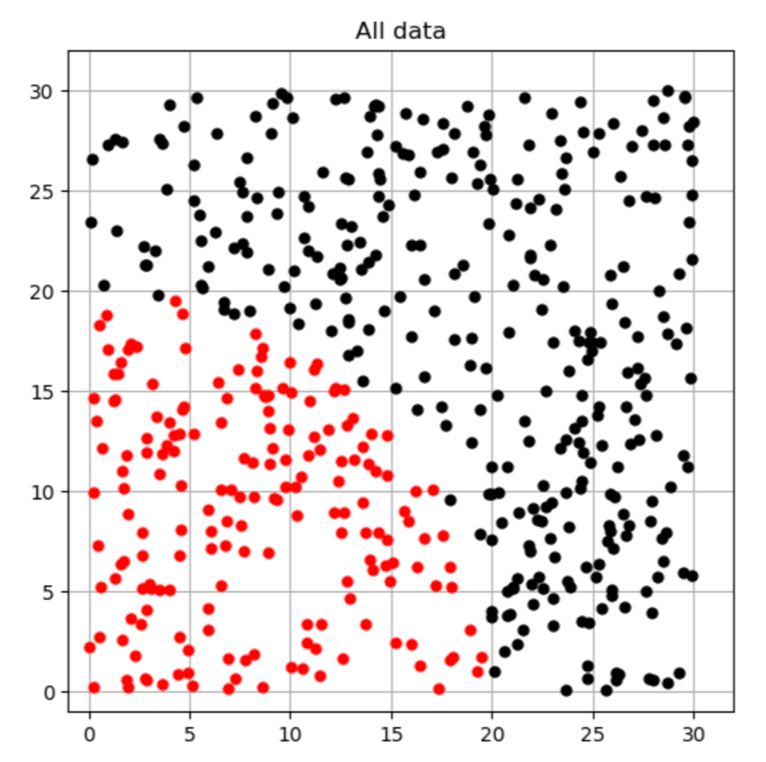
\includegraphics[scale = 0.3]{optimization/figures/figures-static/svm-nonlinear} \ \ \ \ \ 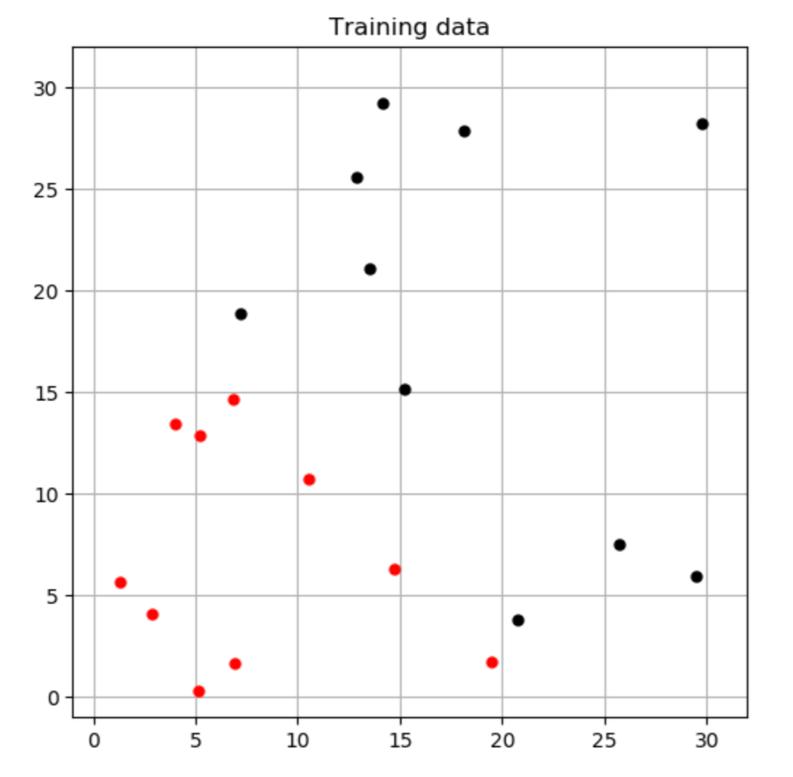
\includegraphics[scale = 0.3]{optimization/figures/figures-static/svm-nonlinear-training}
\end{center}
Here we have a classification problem where the data cannot be separated by a hyperplane.  On the left, we have all of the data given to use.  On the right, we have a subset of the data that we could try using for training and then test our learned function on the remaining data.  As we saw in class, this amount of data was not sufficient to properly classify most of the data.
\end{example}

We cannot learn this classifier from the data directly using the hyperplane separation with SVM in the last section.  But, if we modify the data set, then we can do this.  

For each data point $x$, we transform it into a data point $X$ by adding a third coordinate equal to $x_1^2 + x_2^2$.  That is 
\begin{equation}
x = \begin{pmatrix} x_1 \\ x_2 \end{pmatrix} \quad \rightarrow \quad X = \begin{pmatrix} x_1 \\ x_2 \\ x_1^2 + x_2^2 \end{pmatrix}.
\end{equation}
In this way, we convert the data $x^1, \dots, x^N$ into data $X^1, \dots, X^N$ that lives in a higher-dimensional space.  But with this new dataset, we can apply the hyperplane separation technique in the last section to properly classify the data.

This can be done with other nonlinear classification functions.  

\subsection{Support Vector Machines}





\subsection*{One-Class SVM for Anomaly Detection: An Example in Credit Card Fraud Detection}
The idea behind One-Class SVM is to find the best hyperplane that separates all the data points from the origin (in feature space) and maximizes the distance from this hyperplane to the origin. If a data point falls far from this hyperplane, it can be considered an anomaly.
\paragraph{Problem Statement}

You are given transactional data from a credit card company. The majority of transactions are legitimate, but a small fraction of them are fraudulent. The goal is to detect the fraudulent transactions.

\paragraph{Data}

For each transaction, you have various features:
\begin{itemize}
    \item Amount of the transaction
    \item Date and time
    \item Location
    \item Previous transaction history of the card
    \item Merchant information
\end{itemize}

Given the number of legitimate transactions is much higher than the number of fraudulent ones, this is a highly imbalanced dataset.

\subsubsection*{Steps for Using One-Class SVM}

\begin{enumerate}
    \item \textbf{Data Preparation:}
    \begin{itemize}
        \item Normalize the data since SVMs are sensitive to the scale of the input.
        \item If the data dimension is high, consider dimensionality reduction techniques (e.g., PCA) to make computation more feasible.
    \end{itemize}

    \item \textbf{Training the Model on Normal Data:} 
    Train the One-Class SVM only on the legitimate transactions. The idea is to understand the "shape" of normal data. If a transaction does not fit this shape, it's likely an anomaly.

    \item \textbf{Hyperparameter Tuning:}
    \begin{itemize}
        \item \textbf{Kernel:} Common choices include linear, polynomial, and radial basis function (RBF). The choice of kernel affects the decision boundary.
        \item \textbf{Nu:} This parameter, typically between 0 and 1, sets an upper bound on the fraction of margin errors and a lower bound of the fraction of support vectors.
        \item \textbf{Gamma:} If using the RBF kernel, gamma defines how much influence a single training example has. Low values mean 'far' and high values mean 'close'.
    \end{itemize}

    \item \textbf{Detection:} For each transaction, use the trained One-Class SVM to predict if it's an anomaly. If the SVM classifies it as not belonging to the trained class, it's flagged as an anomaly.

    \item \textbf{Evaluation:} Since the dataset is imbalanced, accuracy might not be the best metric. Instead, focus on metrics like precision, recall, the F1 score, or area under the ROC curve.
\end{enumerate}

\paragraph{Advantages}

\begin{itemize}
    \item Effective in high-dimensional spaces.
    \item Requires only normal data for training, making it suitable for datasets where anomalies are rare and not well-defined.
\end{itemize}

\paragraph{Disadvantages}

\begin{itemize}
    \item Can be sensitive to the choice of hyperparameters.
    \item Might be computationally intensive on large datasets.
\end{itemize}


One-Class SVM provides a way to detect anomalies by learning the distribution of only the normal class and flagging observations that deviate from this. It can be particularly useful in scenarios where anomalies are rare and hard to define.
